\documentclass{mwart}

\usepackage{polski} % Pozwala na użycie polskiego. Ustawia między innymi fontenc na T1
\usepackage[utf8]{inputenc} % Informuje o kodowaniu
\usepackage{enumitem}
\usepackage{xcolor}
\usepackage{xcolor}% http://ctan.org/pkg/xcolor
\usepackage{hyperref}% http://ctan.org/pkg/hyperref
\usepackage{listings}
\usepackage{float}

\lstset{
  basicstyle=\ttfamily,
  columns=fullflexible,
  breaklines=true,
  postbreak=\mbox{\textcolor{red}{$\hookrightarrow$}\space},
}

\definecolor{LinkColor}{HTML}{1d5cc1}

\usepackage{tabto}

\usepackage{graphicx} % Pakiet do obrazów
\graphicspath{ {./Obrazy/} } % Folder, z którego będą brane obrazy

% Nie twórz nowych stron
\usepackage{etoolbox}
\makeatletter
% \patchcmd{\chapter}{\if@openright\cleardoublepage\else\clearpage\fi}{}{}{}
\makeatother

\title{Raport końcowy -- Gra w życie}
\author{Krzysztof Dąbrowski i Jakub Bogusz}
\date{\today}

\begin{document}
\maketitle{}

\tableofcontents{}

\section{Ostateczny projekt modułów}
\paragraph{Zmodyfikowany diagram modułów:}\mbox{}\\
\begin{figure}[H]
	\centering
	\def\svgwidth{\columnwidth}
	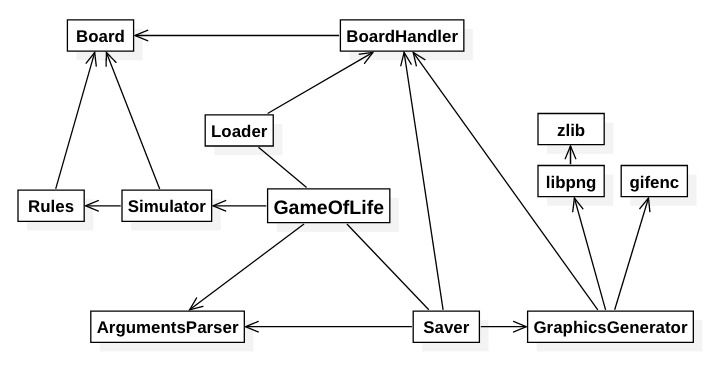
\includegraphics[width=13cm]{diagram_modulow.png}
\end{figure}


%TODO: Ostateczny projekt modułów}

\section{Opis modyfikacji}
%TODO: Opis modyfikacji}

\section{Prezentacja działania}
Przykłady wywołania programu z różnymi flagami.

\subsection{Generacja obrazów z wczytaniem stanu z pliku}
Program wywołany w następujący sposób: \\
\texttt{./game-of-life -f input.txt -t png -o raport -n 6}
Argumenty oznaczają:
\begin{itemize}
\item \texttt{-f input.txt} -- Stan początkowy jest wczytany z pliku ,,input.txt'',
\item \texttt{-t png} -- Zostanie wygenerowana seria plików .png z kolejnymi pokoleniami,
\item \texttt{-o raport} -- Wygenerowane pliki zostaną zapisane do folderu ,,raport'',
\item \texttt{-n 6} -- Zostanie wygenerowanych 6 następnych pokoleń .png (ze stanem początkowym 7 obrazków).
\end{itemize}


%TODO: Prezentacja działania}

\section{Podsumowanie testów modułów}
%TODO: Podsumowanie testów modów}

\section{Analiza pamięci}
\noindent Raport programu \texttt{valgrind } zwraca następujące wyniki:\\\\
\noindent \texttt{\noindent 
==18728== LEAK SUMMARY:\\
==18728==    definitely lost: 0 bytes in 0 blocks\\
==18728==    indirectly lost: 0 bytes in 0 blocks\\
==18728==      possibly lost: 72 bytes in 3 blocks\\
==18728==    still reachable: 23,728 bytes in 28 blocks\\
==18728==         suppressed: 18,077 bytes in 153 blocks\\
\\
==18728== ERROR SUMMARY: 0 errors from 0 contexts 
}\\\\

2 pierwsze linie raportu informują o braku definitywnych wycieków pamięci, co oznacza że program prawidłowo zarządza pamięcią.

Wycieki oznaczone jako \texttt{still reachable} oraz \texttt{possibly lost} spowodowane są przez funkcje bibliotek \texttt{ctime} oraz \texttt{libpng}, więc nie mamy na nie wpływu i nie jesteśmy w stanie ich wyeliminować. Załączamy fragmentu raportu opisujące te wycieki:\\

\paragraph{possible leaks:} \mbox{}

\begin{scriptsize}
\noindent \texttt{\noindent 
\\==18752== 72 bytes in 3 blocks are possibly lost in loss record 34 of 60
\\==18752==    at 0x1000B26EA: calloc (in /usr/local/Cellar/valgrind/3.14.0/lib/valgrind/vgpreload\_memcheck-amd64-darwin.so)
\\==18752==    by 0x1007AD7C2: map\_images\_nolock (in /usr/lib/libobjc.A.dylib)
\\==18752==    by 0x1007C04E0: map\_images (in /usr/lib/libobjc.A.dylib)
\\==18752==    by 0x10000DC64: dyld::notifyBatchPartial(dyld\_image\_states, bool, char const* (*)(dyld\_image\_states, unsigned int, dyld\_image\_info const*), bool, bool) (in /usr/lib/dyld)
\\==18752==    by 0x10000DE39: dyld::registerObjCNotifiers(void (*)(unsigned int, char const* const*, mach\_header const* const*), void (*)(char const*, mach\_header const*), void (*)(char const*, mach\_header const*)) (in /usr/lib/dyld)
\\==18752==    by 0x10027871D: \_dyld\_objc\_notify\_register (in /usr/lib/system/libdyld.dylib)
\\==18752==    by 0x1007AD073: \_objc\_init (in /usr/lib/libobjc.A.dylib)
\\==18752==    by 0x100202B34: \_os\_object\_init (in /usr/lib/system/libdispatch.dylib)
\\==18752==    by 0x100202B1B: libdispatch\_init (in /usr/lib/system/libdispatch.dylib)
\\==18752==    by 0x1001119C2: libSystem\_initializer (in /usr/lib/libSystem.B.dylib)
\\==18752==    by 0x10001FAC5: ImageLoaderMachO::doModInitFunctions(ImageLoader::LinkContext const\&) (in /usr/lib/dyld)
\\==18752==    by 0x10001FCF5: ImageLoaderMachO::doInitialization(ImageLoader::LinkContext const\&) (in /usr/lib/dyld)
}
\end{scriptsize}
\\

\paragraph{still reachable:}\mbox{}

\begin{scriptsize}
\noindent \texttt{\noindent 
\\==18805== 18,280 bytes in 1 blocks are still reachable in loss record 60 of 60
\\==18805==    at 0x1000B26EA: calloc (in /usr/local/Cellar/valgrind/3.14.0/lib/valgrind/vgpreload\_memcheck-amd64-darwin.so)
\\==18805==    by 0x100351930: tzsetwall\_basic (in /usr/lib/system/libsystem\_c.dylib)
\\==18805==    by 0x1003537C9: localtime (in /usr/lib/system/libsystem\_c.dylib)
\\==18805==    by 0x100353945: ctime (in /usr/lib/system/libsystem\_c.dylib)
\\==18805==    by 0x1000039AF: setup (Saver.c:5)
\\==18805==    by 0x100003A2E: saveCommon (Saver.c:12)
\\==18805==    by 0x100003E59: saveAsPng (Saver.c:53)
\\==18805==    by 0x10000405E: runProgram (main.c:83)
\\==18805==    by 0x100003F31: main (main.c:32)
}
\end{scriptsize}




%TODO: Analiza pamięci

\end{document}


